\documentclass[letterpaper]{article}

%% Language and font encodings
\usepackage[english]{babel}
\usepackage[utf8x]{inputenc}
\usepackage[T1]{fontenc}

%% Sets page size and margins
\usepackage[letterpaper,top=3cm,bottom=2cm,left=2cm,right=2cm,marginparwidth=1.75cm]{geometry}

%% Useful packages
\usepackage{amsmath}
\usepackage{graphicx}
\usepackage[colorinlistoftodos]{todonotes}
\usepackage[colorlinks=true, allcolors=blue]{hyperref}
\usepackage{listings}
\usepackage{enumitem}

\usepackage[numbered,framed]{matlab-prettifier}
\let\ph\mlplaceholder % shorter macro
\lstMakeShortInline"

\lstset{
  style              = Matlab-editor,
  basicstyle         = \mlttfamily,
  escapechar         = ",
  mlshowsectionrules = true,
}

\title{EE576 HW 6}
\author{Jordan Caudill and Matt Ruffner}

\begin{document}
\maketitle

%%%%%%%%%%%%%%%%%%%%%%%%%%%%%%%%%%%%%%%%%%%%%%%%%%%%%%%%%%%%%%%%%%
%%%%%%%%%%%%%%%%%%%%%%%%%%%%%%%%%%%%%%%%%%%%%%%%%%%%%%%%%%%%%%%%%%
%%%%%%%%%%%%%%%%%%%%%%%%%%%%%%%%%%%%%%%%%%%%%%%%%%%%%%%%%%%%%%%%%%

\section{Part 1}

\begin{enumerate}
    \item The IP address of the DNS server is \texttt{10.1.1.3}
    \item The status is \texttt{NOERROR}
    \item The IP address of \texttt{www.google.com} is \texttt{10.1.2.155}
    \item The cache time is 10 seconds
    \item The authoritative name server for \texttt{www.google.com} is \texttt{ns.google.com}
    \item The authoritative name sever IP address is \texttt{10.1.2.3}.
\end{enumerate}

\section{Part 2}

The network topology is shown in Fig. \ref{fig:topo} for reference.
\begin{figure}[h!]
    \centering
    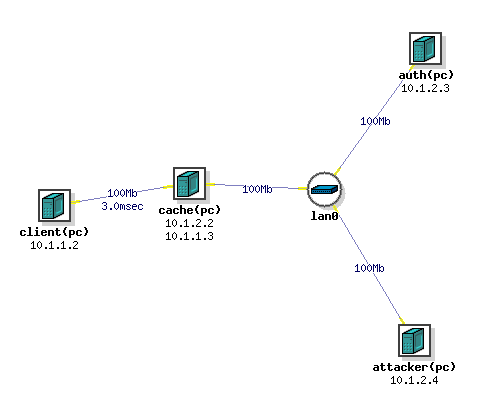
\includegraphics[width=5cm]{images/hw7topo}
    \caption{Topology of the DeterLab network setup.}
    \label{fig:topo}
\end{figure}

\section{Part 3}

\section{Part 4}





\end{document}